\section{研究背景}
\begin{comment}
%%%%%以下コメントアウト済み%%%%%
%TODO 渡邊先輩の緒言をもとに書き改める
ヒトの運動制御を理解することは,ヒトの運動機能への介入や調和を目指すロボットの開
発にとって極めて重要である.例えば,患者と相互に関わりながら運動機能の再獲得を促す
リハビリテーションロボットは,より効率的な効果を上げるために,ヒトの運動戦略に基づ
きながらトレーニングすることが望まれる.また,ヒトのような柔軟かつ滑らかな運動を実
現することを目指す筋骨格ロボットの開発において,ヒトの骨格や運動制御を規範としてロ
ボットのシステムに応用することは有望な方法である.これらのロボットを実現するために,
ヒトの骨格の仕組み及び運動戦略を明らかにすることは不可欠である.

本研究は,日常的な拘束運動であるペダリングの運動戦略を筋協調・平衡点・メカニカル
インピーダンスの観点から明らかにする.明らかになった戦略に基づき筋骨格ロボットの制
御を行い,解析結果の検証及びロボット制御への応用を模索する.
\end{comment}

ヒトの運動制御を理解することにより,ヒトの運動機能への介入や調和を目指したロボットの
開発がより行われやすくなる.例えば,患者と相互に関わりながら運動機能の再獲得を促す
リハビリテーションロボットは,より効率的な効果を上げるため,ヒトの運動戦略に基づきながら
トレーニングすることが望まれる.また,ヒトのような柔軟かつ滑らかな運動を実現することを
目指す筋骨格ロボットの開発において,ヒトの骨格や運動制御を規範としてロボットのシステムに
応用することは非常に有望な方法であると考えられている.これらのロボットの実現をするため,
ヒトの骨格の仕組みや運動戦略を明らかにすることは不可欠である.

また,近年,ロボットの社会進出は凄まじさを増しており,街中でもロボットを見かける様になった.
そのような環境の中,旧来からのハードなロボットではなく伸縮性や柔軟性に優れた,ソフトロボットの
研究開発が盛んに行われるようになった.ソフトロボットはその伸縮性や柔軟性を生かし助長性の高い,
動作を行うことができるようになった.更に,これらに合わせて,ロボットの動作を計測するセンサも
柔軟なものとなる必要性が出てきた.

本研究はそのような研究背景の元,行われたものとなっている.

\section{先行研究例}

\subsection{フレキシブルストレッチセンサ}%TODO:伸縮センサのお話を書く
ロボットの社会進出に伴い、ハードなロボットではなく柔軟性を持ったやわらかロボットの研究開発が
盛んに行われている。その様な中、ロボットの動作の計測を行うセンサーも柔軟性を持つ必要性が増加している。
導電性ゴムを利用した伸縮センサの開発が行われ実際に販売されているが、高価であり既製品であるため、センサー長が
定まったもののみとなっている。

soft robotics toolkit\cite{MITSoftRobot}において,シリコンと導電性布をもちいた自作できる伸縮センサが
紹介されている.本センサは,伸縮性に優れており,柔軟性も兼ね備えたものとなっている.また,
製作コストも\$23と非常に安価なものであると紹介されている.

今回は,このような安価で自作することのできるセンサーとその計測系を作成し,
本センサーを空気圧人工筋を用いた足関節ロボットに搭載し,空気圧人工筋の伸展の計測を行うことを目標とする.
\begin{figure}[h]
    \begin{center}
        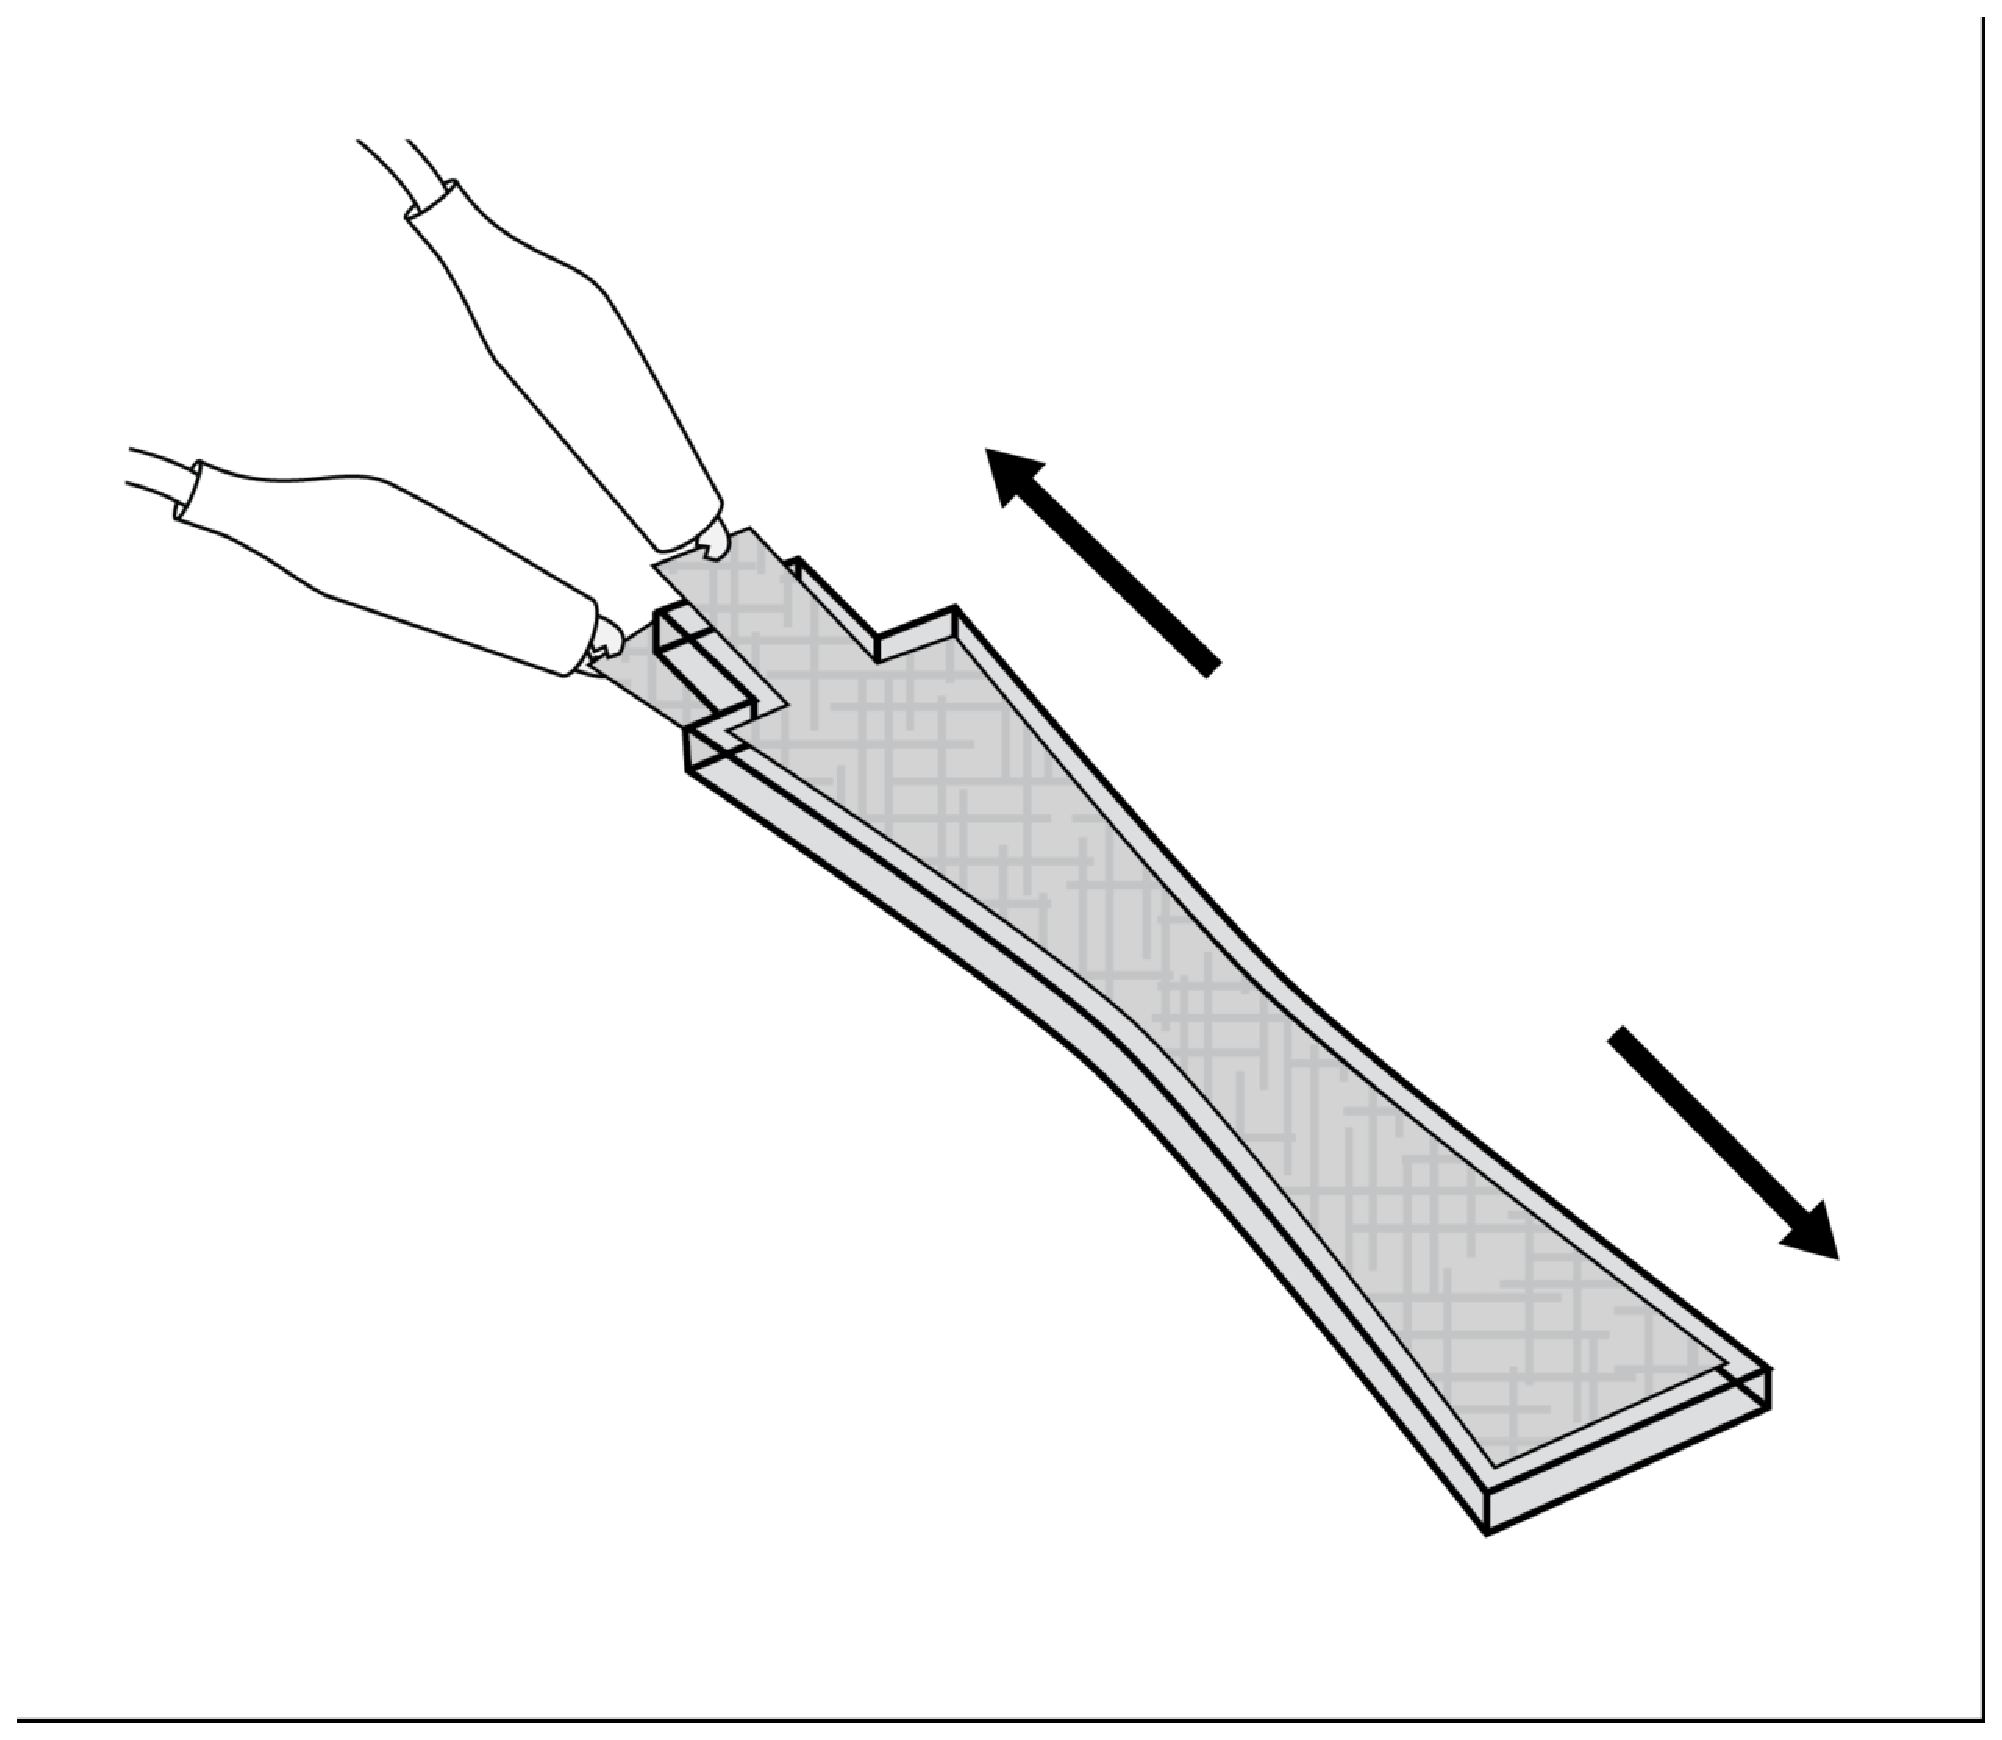
\includegraphics[width=0.5\columnwidth]{./1_prolusion/MITSoftRobotics.eps}
        \caption{伸縮センサ模式図\cite{MITSoftRobot}}
        \label{MITSoftRobot表紙}
    \end{center}
\end{figure}

\subsection{ペダリングロボット}
%TODO:初号機体のお話を書く
%TODO:初号機関連の研究のリファレンスを貼る
%TODO:奥先輩の論文を貼る

先行研究として,人間の筋肉を模した空気圧人工筋をもちいたペダリングロボットが存在する.
これは,人間のペダリング動作における筋シナジーの計測を行い,ロボットに再現させるものであった.
筋シナジーの計測は片麻痺患者,健常者ともに行い,片麻痺患者におけるペダリング動作時の特徴的な
活動状態を健常者との比較で行った.ヒトの運動解析を行い,運動戦略を明らかにするために製作され
使用されたロボットである.本ロボットは,腰がサドル上に固定された状態で股関節,膝関節,足関節
それぞれがピッチ方向にのみ自由度を持っており2次元平面上における動作を再現することが出来た.
これらの動作を再現するために,空気圧人工筋がヒラメ筋,前脛骨筋,大腿四頭筋,大腿二頭筋,腸腰筋,恥骨筋の
6筋分が搭載された形となっている.なお,空気圧人工筋の出力上,日本人成人男性の半分の重量モデルで作製さている.%TODO:筋肉の数をちゃんと確認する
\begin{figure}[h]
 \begin{center}
  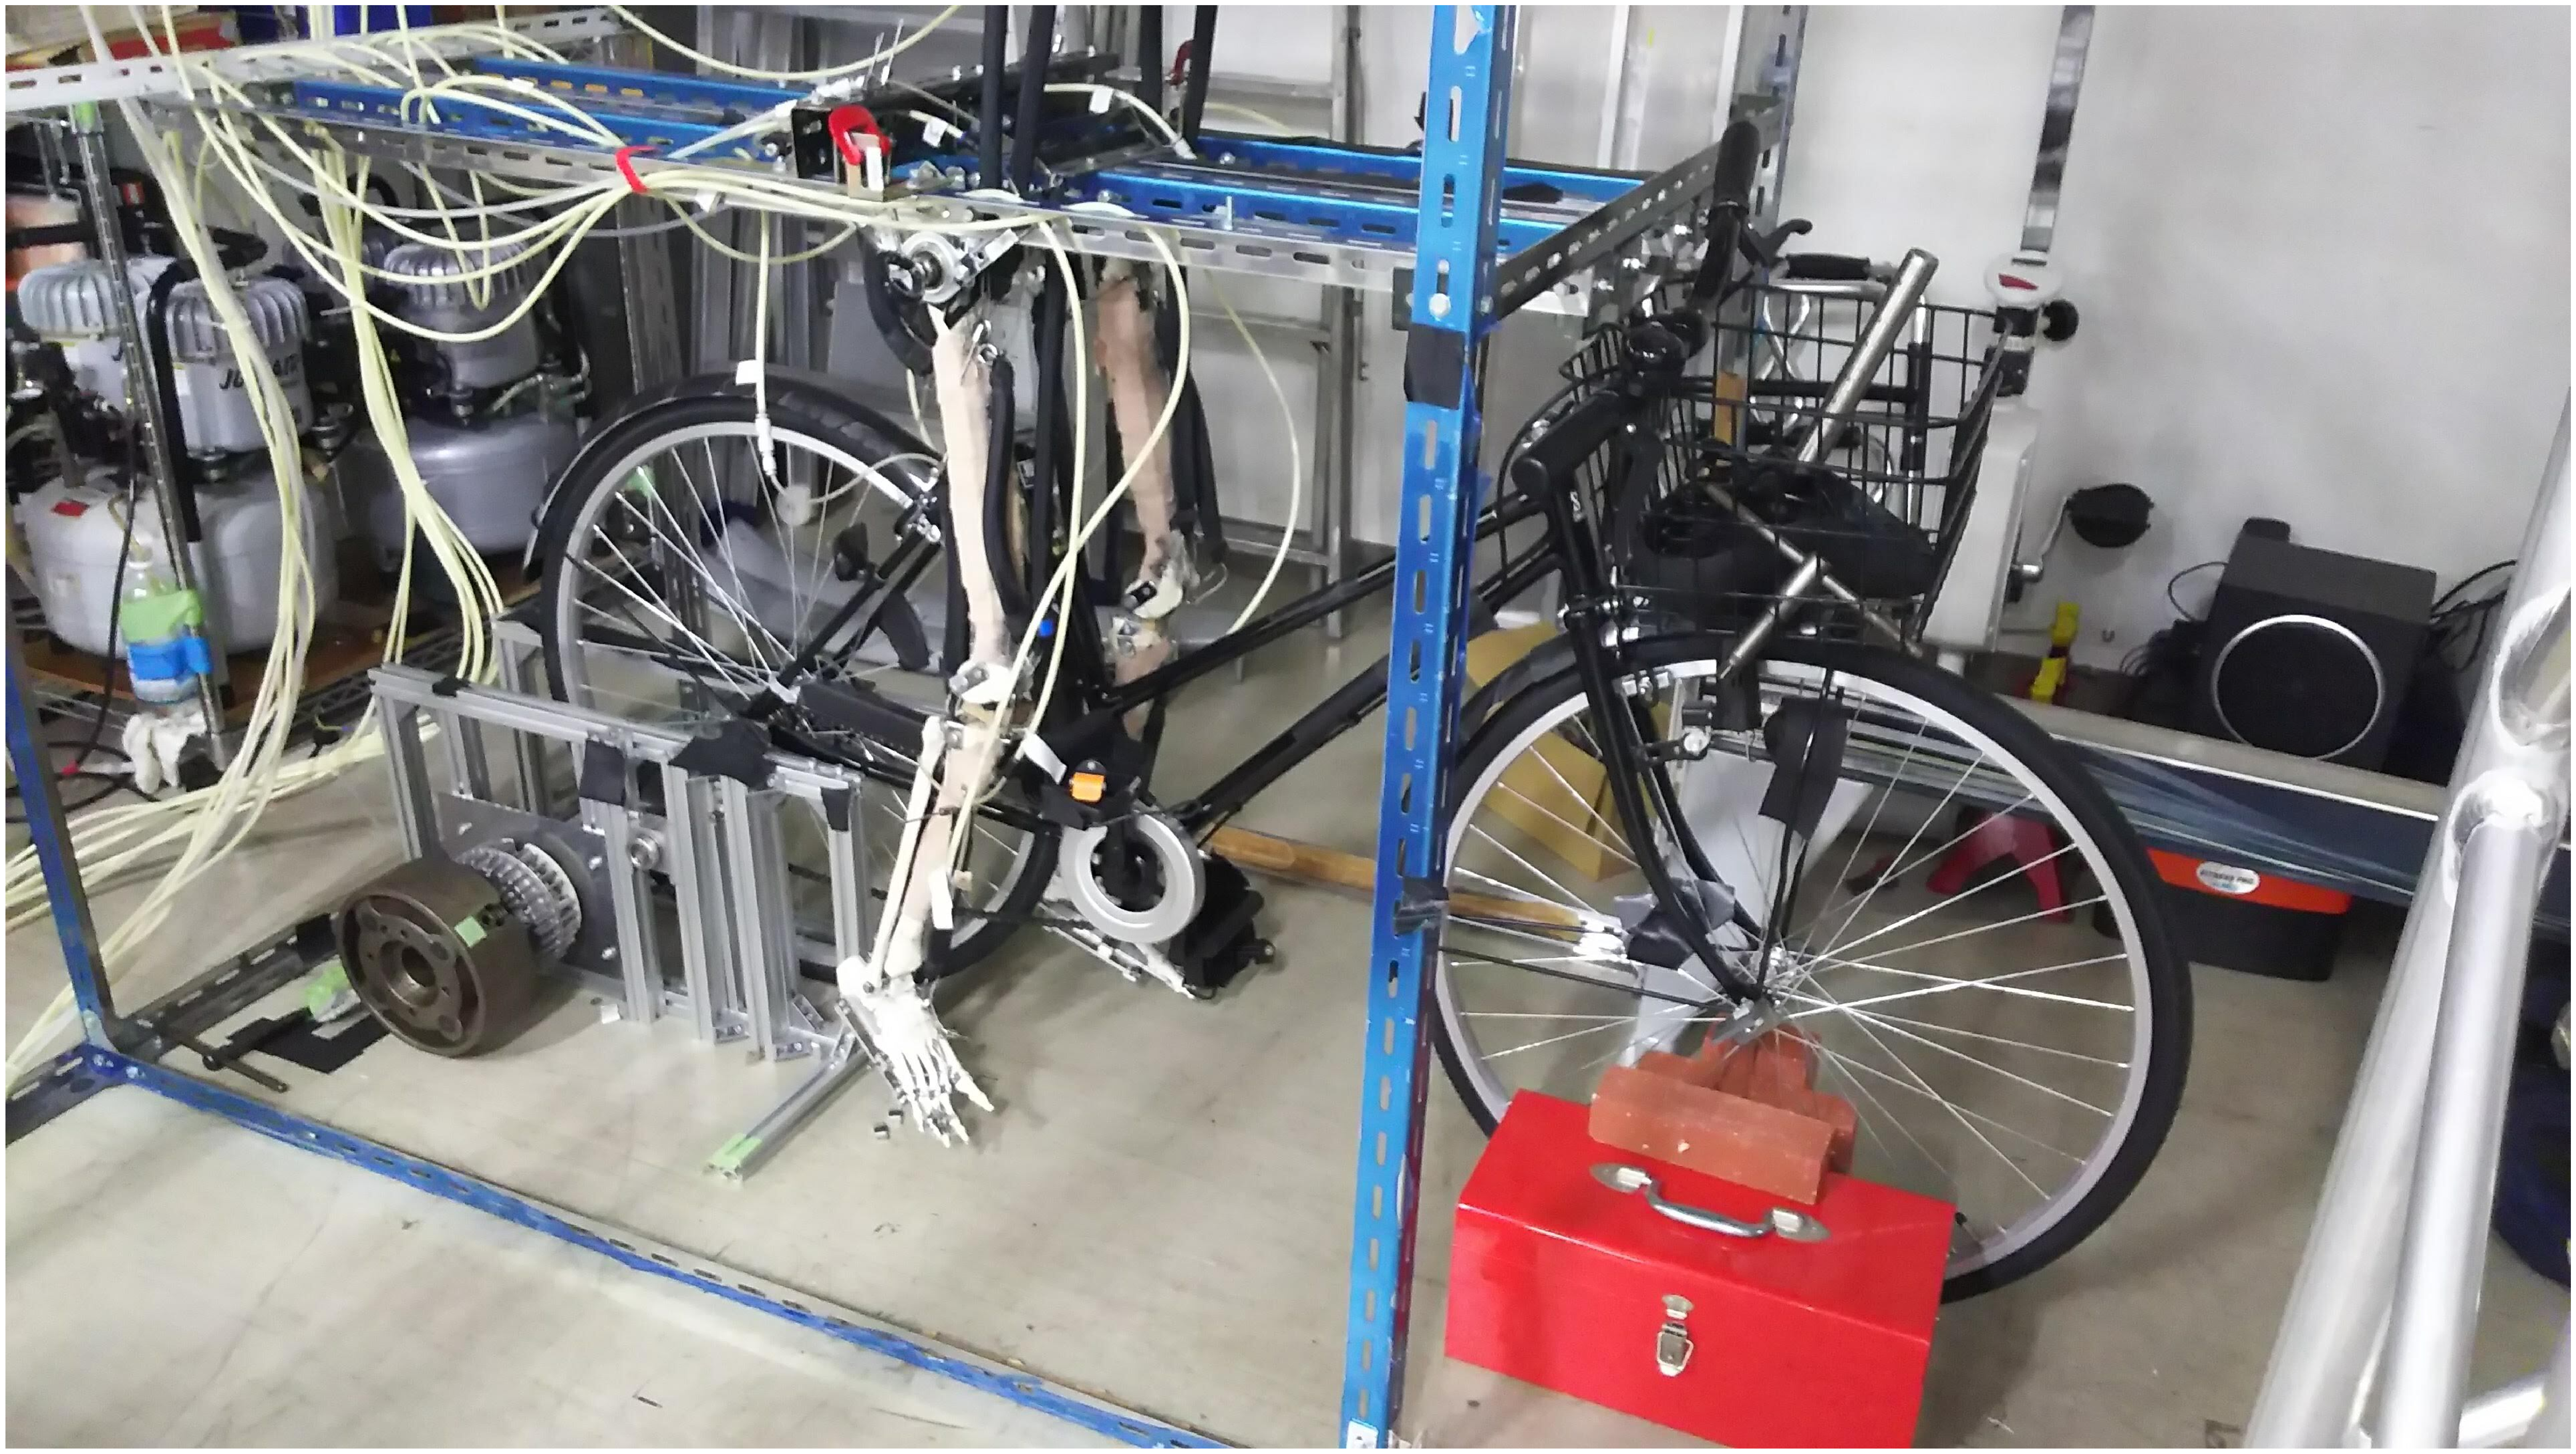
\includegraphics[width=0.75\columnwidth,clip]{./1_prolusion/1st.eps}
  \caption{ペダリングロボット}
  \label{初号機}
  \end{center} %
\end{figure}

\newpage

\subsection{二足歩行ロボット}
%TODO:2号機のお話を書く
%TODO:2号機関連の研究のリファレンスを貼る
先述のペダリングロボットの研究成果を生かし、腰椎を固定していない状態の二足歩行ロボットが製作された。
本ロボットは、腰椎が固定されていないことにより立脚時の歩容動作の再現を行えるようになった。
なお、動作時は自重を支えることができないため、股間部の支持を行った。また、関節動作に関しては
先述のロボットと同様の形となっており,股関節,膝関節,足首関節それぞれがピッチ方向にのみ自由度を持っており
2次元平面上における動作を再現することが出来た.これらの動作の再現を行うため、空気圧人工筋が
ヒラメ筋,前脛骨筋,大腿四頭筋,大腿二頭筋,腸腰筋,恥骨筋の6筋分が搭載された形となっている.

これらの研究によって平衡点仮説に基づく筋シナジー解析を用いた歩行動作の解明の為に用いられた。
この歩行動作解析により、健常者の歩行と片麻痺患者の歩行の動作の相違に関して解明することができた。
\begin{figure}[h]
  \begin{center}
  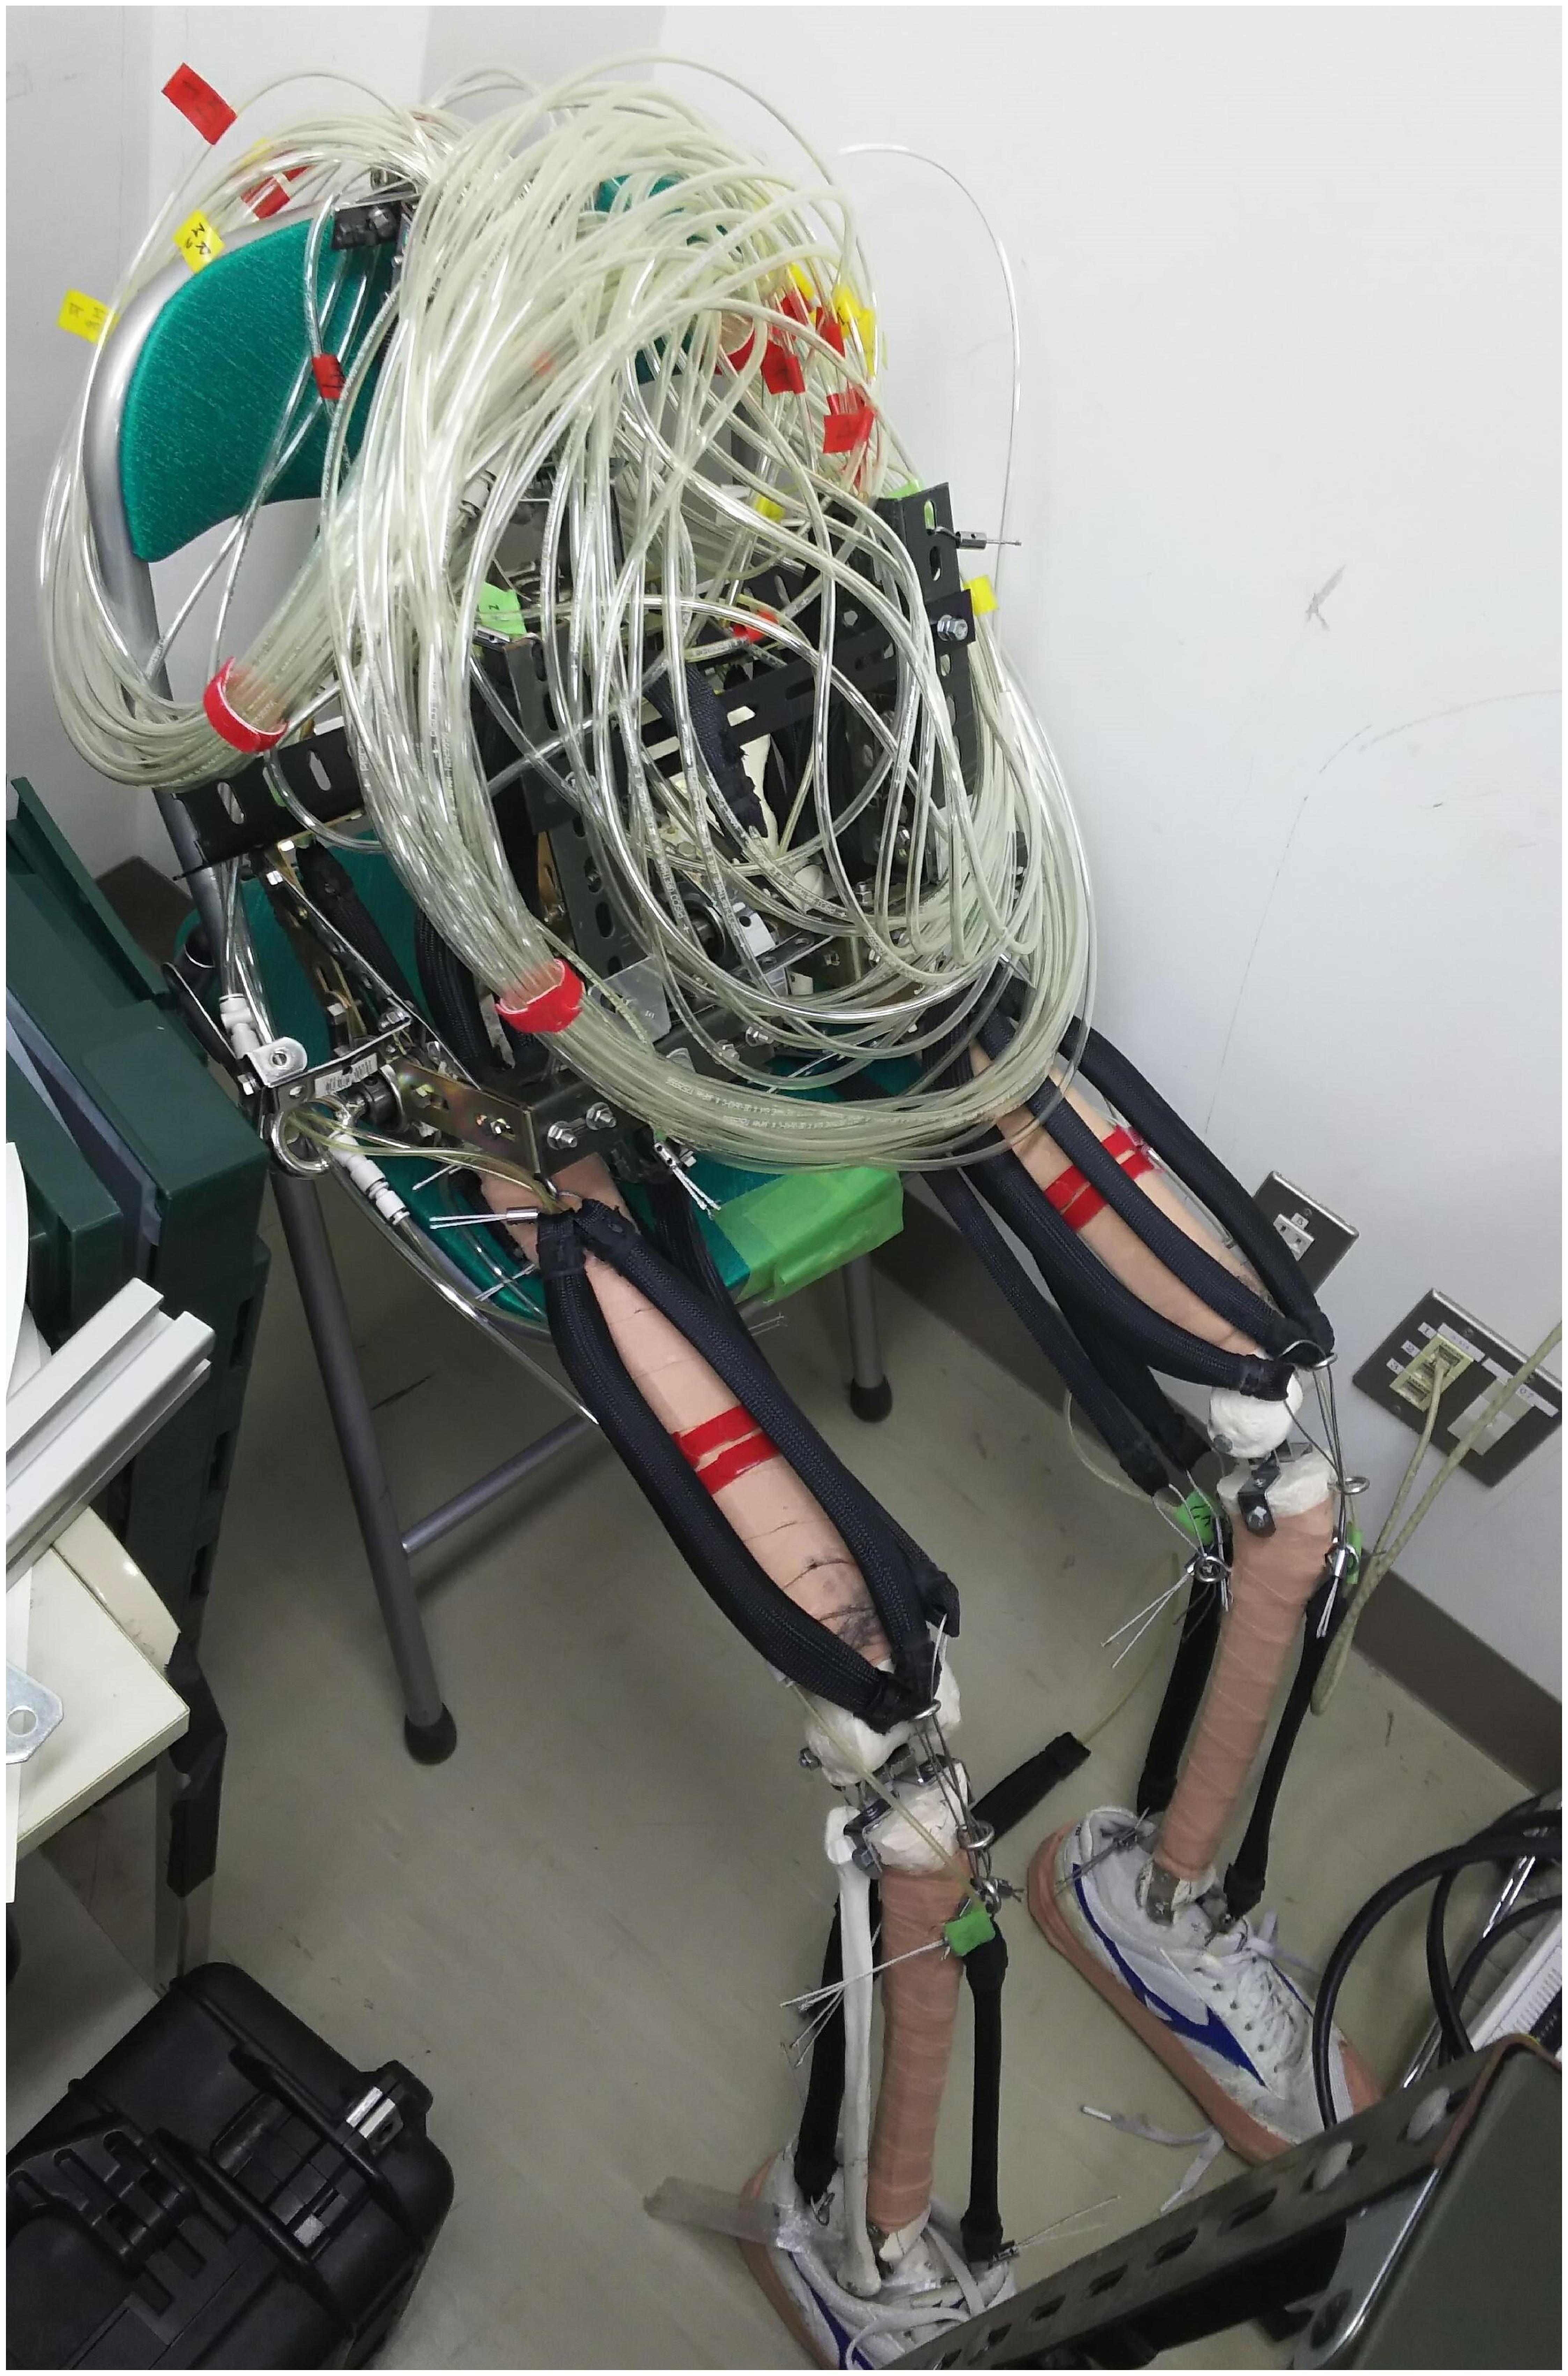
\includegraphics[width=0.35\columnwidth,clip]{./1_prolusion/2nd.eps}
  \caption{二足歩行ロボット}
  \label{2号機}
 \end{center}
\end{figure}

\newpage

\section{研究目的}
%TODO:これらを統合し,筋肉の伸長を巻き込んだシステムの話をする
先述の先行研究例を踏まえ、やわらかいアクチュエータである空気圧人工筋の伸長計測をフレキシブルストレッチセンサを用いて計測を
行うことを一つの目的とする。そのために、導電性布を用いたフレキシブルストレッチセンサの製作を行った。また、センサ自体を自作するため、
本センサの計測系の設計製作も行った。

また、ペダリングロボット,2足歩行ロボットの経験を踏まえ,新たに足関節ロボットの製作を行った。
これは、従来のロボットでは足関節部分の自由度がピッチ方向のみの1自由度であり、動作空間が2次元平面のみに制限されていた。
一方で実際の人間の自由度はこれに加えてロール方向,ヨー方向も存在し3自由度である.
3自由度にすることで平面動作だけでなく空間的な動きも可能になる。
加えて自由度の増加により、前後方向の移動だけでなく、横方向への移動も可能となり人間動作の再現性が向上するとも考えられる。

最終的に、導電性布を用いたストレッチセンサと新たに製作した足関節ロボットを用いて、人間の筋の伸長を計測することを、研究の最終目的とする。

\section{論文構成}
本論文の構成は以下の通りである.
{\bf 第2章}で足関節ロボット、伸縮センサの製作過程と伸縮センサにおけるデータ処理について述べ,{\bf 第3章}でその解析結果を示す.
{\bf 第4章}では考察する. %TODO考察内容の記述を行う
最後に{\bf 第5章}で本論文の成果をまとめる.
